Detection marker is a $15\times13$ 200 mm pattern that is used to determine the pose of a system placed in the workcell using the \hyperref[acro:VISOR]{VISOR}\textsuperscript{\textregistered} vision sensor
mounted on the \hyperref[acro:KR]{KR}. The pose represents the position and orientation in \hyperref[acro:3D]{3D} space. In total, there are ten markers in the robotic workcell.
One each for bending machine unit and unloading station; and ten markers for the storage station.

\begin{figure}[h]
    \centering
    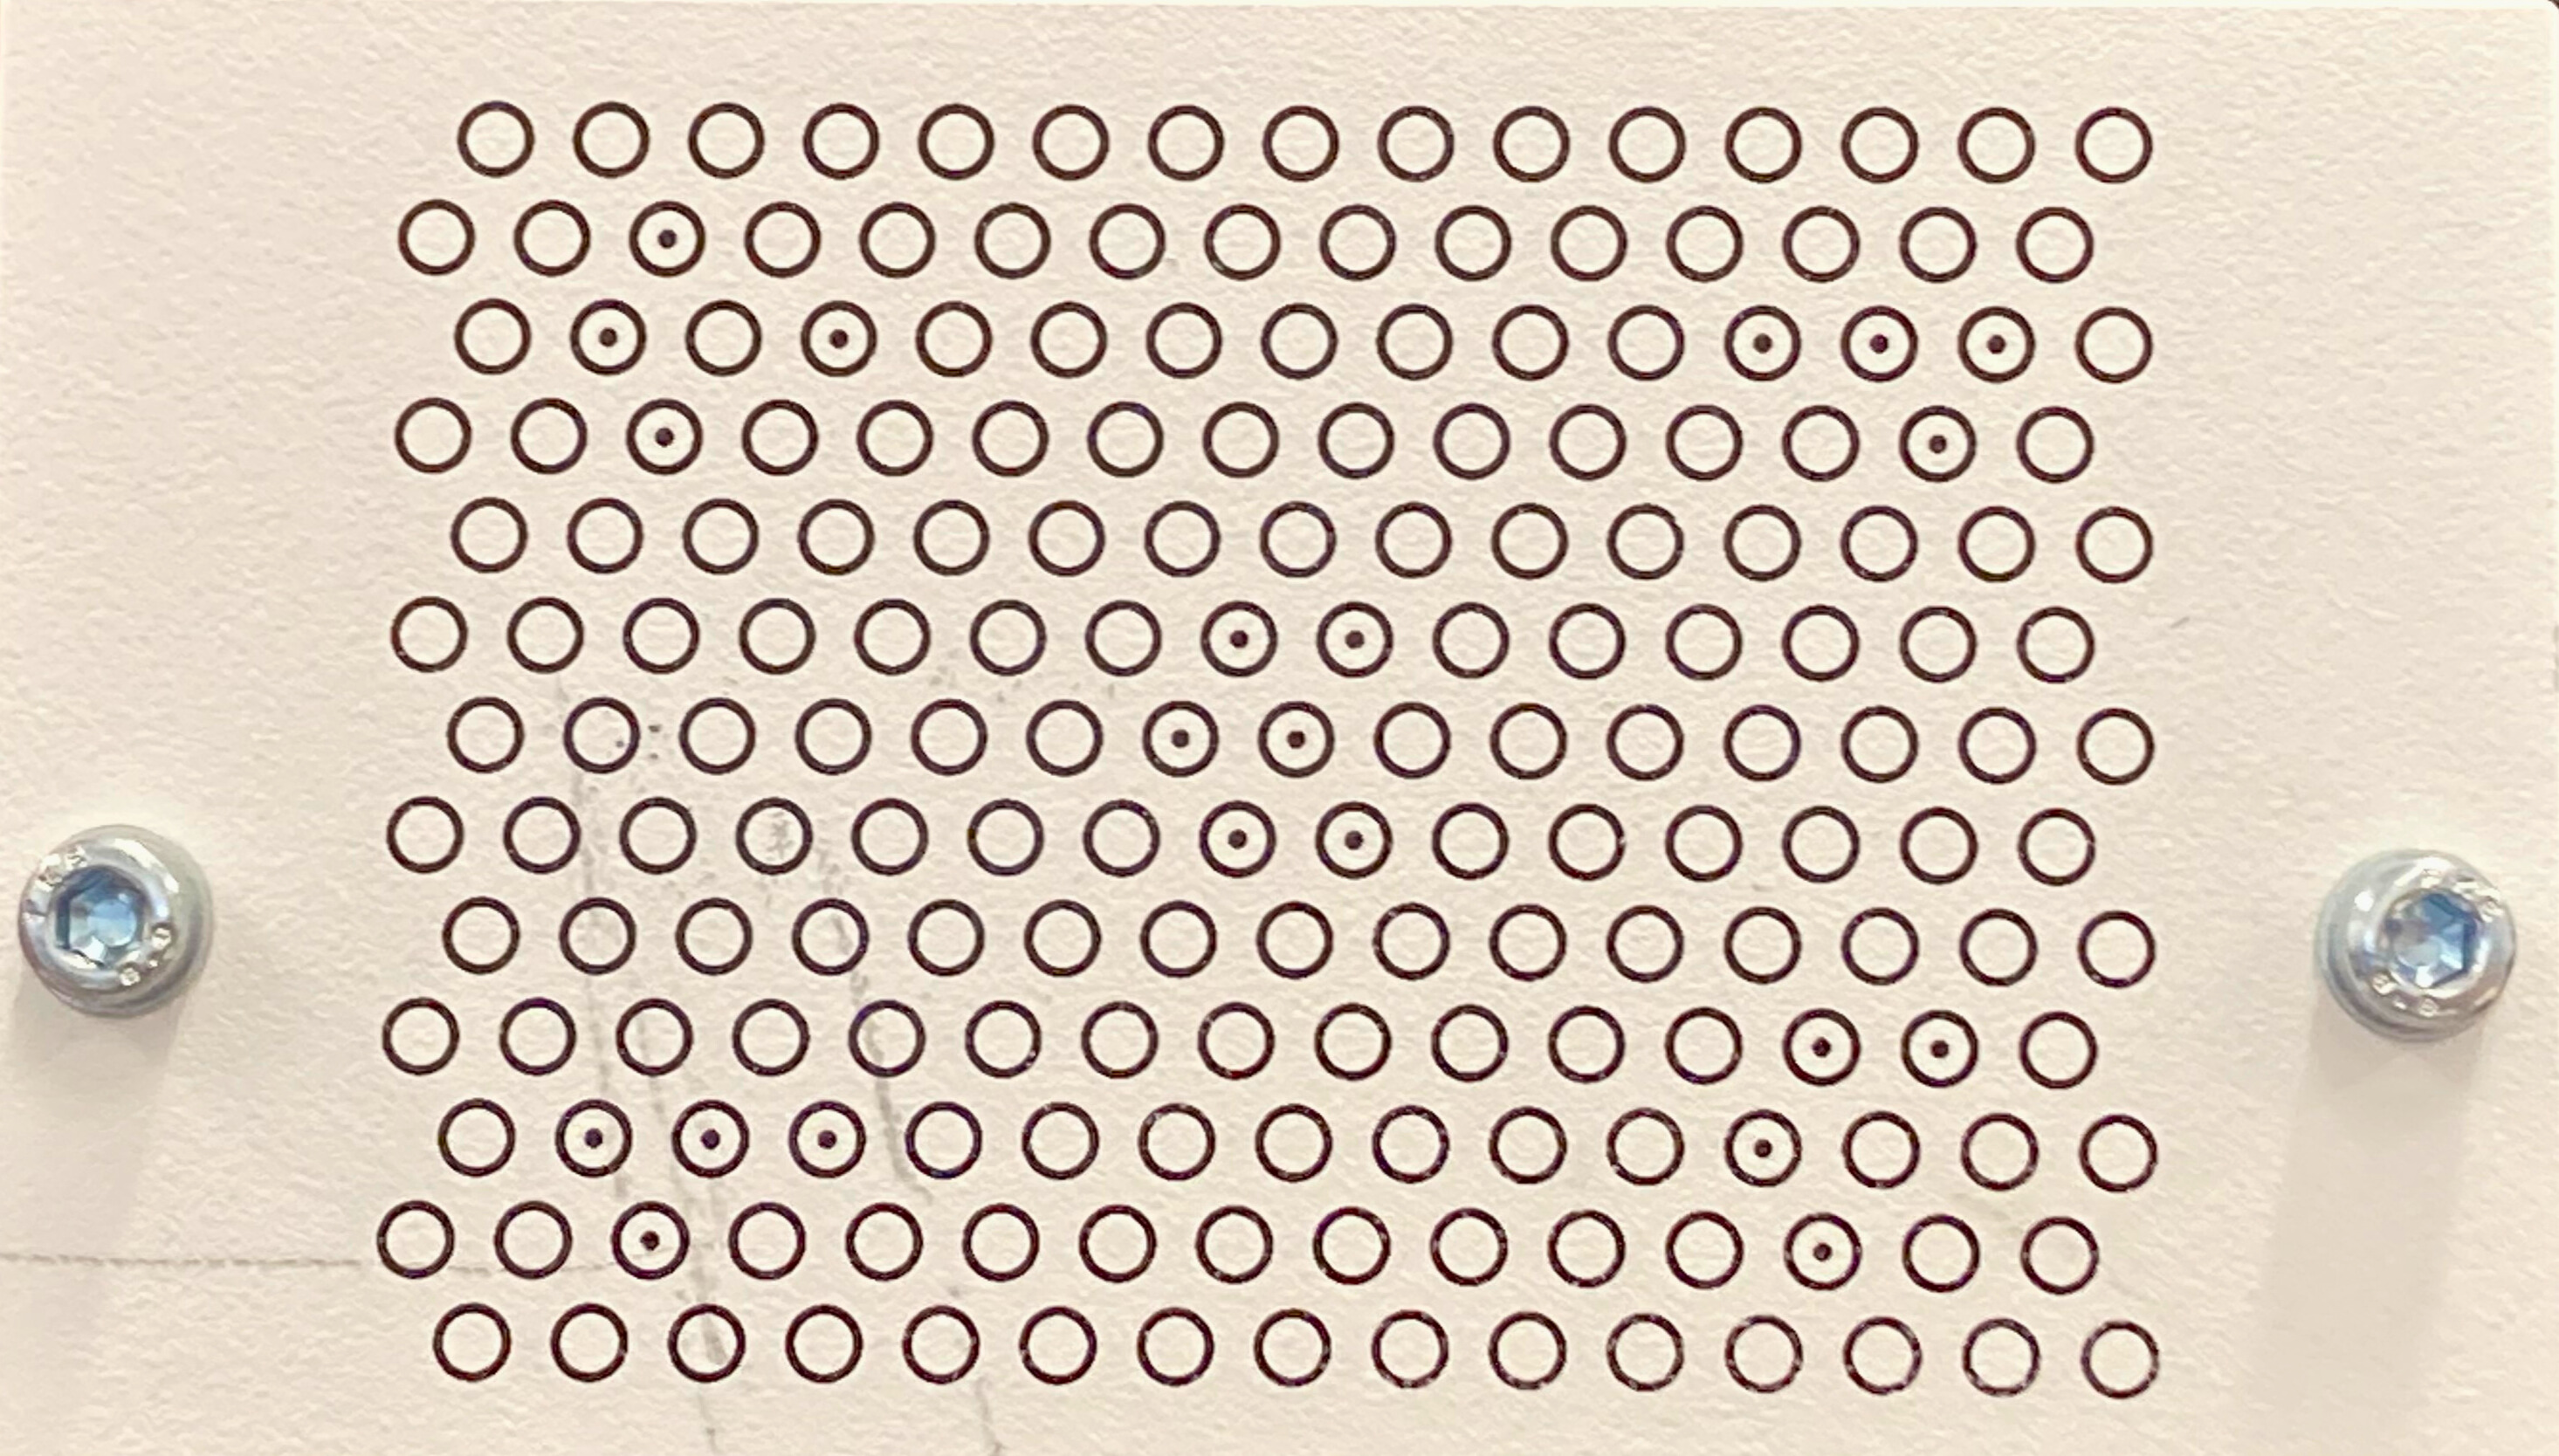
\includegraphics[width=0.5\textwidth]{figures/detection-marker.png}
    \caption{Detection marker}
    \label{fig:marker}
\end{figure}

In addition to get the pose, detection marker is used as calibration plate for auto calibration of camera \textit{w.r.t.} \hyperref[acro:TCP]{TCP}.
